\chapter{Design}
\label{sec:design}

% \vb{ A possible notation is to use capital letters for tuples and small letters otherwise. Header $H$, Content $C$, Block $B=(H,C)$.
% $H=(P,n,D)$, $P$ is the content, $n$ is nonce and $D$ is $\texttt{digest}(C)$.
% Tx block $B^T$, Tx header $H^T$, Tx parent $P^T$, Tx digest $D^T$ and Tx content $C^T$ (similar for prop. and voter block). $B \in \{B^T, B^P, B^V\}$ and so on..}

\section{Notation}
\label{sec:blocktypes}
Each block $B=(H,C)$ is a tuple containting a header $H$ and content $C$.
As discussed in  \S\ref{sec:overview}, there are three types of blocks: transaction blocks, proposer blocks,  and voter blocks.
In all three types, the header $H=(P, n, D)$ is a tuple containing: (1) the hash $P$ of the parent block,
%(\vb{conceptually parent blocks also differ}) \ma{seems ok to me} 
(2)  a valid PoW nonce $n$, and (3) a content digest $D=\texttt{Digest}(C)$. % proving that the block was mined in the correct category (transaction, proposer, or voter). 
We add a superscript to the above notations to denote the type of block being referred. 
For example, we refer  to proposer blocks by $B^P$, transaction blocks by $B^T$, and voter blocks by $B^V$.
% Along the same lines, a proposer block's header, content, and parent are denoted by $H^P$, $C^P$, and $P^P$, respectively, and its content digest by $D^P$.

% The nonce $n$ and content digest $D$ are explained further in the mining procedure (\S\ref{sec:mining}).

%\todo{I intentionally did not  describe what is actually done in the code w.r.t. parent blocks because I think it may confuse people more. Let me know what you think.}
% \ma{I think this is at the right level}

%\paragraph{Transaction blocks.}
% \smallskip
% \noindent{\bf Transaction blocks.}
% Transaction blocks do not need a parent block,  so  $P^T=\emptyset$.
% The content of a transaction block is an ordered list of transactions: $C^T := [t_1, \ldots, t_m]$.
% drawn from the miner's local a memory pool \texttt{mempool} of transactions that have not yet been  incorporated into a transaction block.
% Note that a transaction $t$ is a payment from a sender's public key to a recipient's public key, signed by the sender. 
% \gw{Do we want to mention about multiple senders and recipients?}


% They contain a list of transactions, and a pointer to a parent proposer block. \ma{why do transaction blocks need a pointer to a proposer block? this is also not shown in in Fig. 4} \ma{It might be useful to define a transaction, e.g., it is a payment from a sender public key to a recipient public key, signed by the sender}

% \vb{Below we have described both the content and the mining procedure of the proposer and voter blocks. We can explicitly state that perhaps} \ma{I think this is ok} 

% \smallskip
% \noindent{\bf Proposer blocks.}
% Since the proposer tree is built in a longest-chain fashion, proposer blocks choose as their parent $P^P$  the tip of the longest chain in the proposer tree. 
% Each proposer block's content, $C^P$, is an ordered list of references to other proposer and/or transaction blocks.  
% We compute $B$'s set of \emph{ancestors} by following the chain of parent links in the proposer tree.
% For proposer block $B$, let $C^P_1 =[B^P_{i_1}, B^P_{i_2}, \ldots]$ denote an ordered list of proposer blocks that are neither indirectly referenced or among content of $B$'s ancestors.
% Let $C^P_2 = [B^T_{j_1}, B^T_{j_2},\ldots]$ denote an ordered list of transaction blocks that are not referenced (directly or indirectly) by any of $B$'s ancestors or by any of the proposer blocks in $C^P_1$.
% The content of the proposer block is the concatenation of these two ordered lists: $C^P  :=(C^P_1, C^P_2)$.
% Note that $C^P$ actually stores references to the listed blocks, but we describe them as blocks here to reduce notation.
% Honest nodes mine proposer blocks on the longest chain in the proposer blocktree, but the longest chain does not determine the final confirmed sequence of proposer blocks, known as the  \emph{leader sequence}. 
% We define the \emph{level} of a proposer block as its distance from the genesis block (Figure \ref{}), and the \emph{height} of the proposer tree as the maximum level that contains any proposer blocks. 
% The confirmed leader sequence of proposer blocks contains one block at every level up to the height of the proposer blocktree, and is  determined by the \emph{voter trees}. 
% \smallskip
% \noindent{\bf Voter blocks.}
% There are $m$ voter trees, where $m \gg 1$ is a fixed parameter chosen by the system designers. 
% The $i^{th}$ voter tree is comprised of voter blocks that are mined on the longest chain of the voter tree. 
% Voter trees are also  built in a longest-chain fashion,  so for a voter block  $B^{V_i}$ in the $i^{th}$ voter tree,  its parent $P^{V_i}$ is the tip of the longest chain in the $i^{th}$ voter tree.
% The block's contents $C^{V_i}$ are a list of references to proposer blocks, or \emph{votes}.
% Recall that the \emph{level} of a proposer block denotes its distance from the genesis block, and the \emph{height} $h$ of the proposer tree is the maximum level that contains any proposer blocks.
% Let $L=\{1,\ldots, h\}$ denote the set of all levels in the proposer blocktree.
% Voter trees are built in a longest-chain fashion; each voter tree's longest chain is allowed to vote at most once on any level in  $L$.
% For a voter block $B^V$, let $\ell'_{B}$ be the latest level of proposer block voter by $B^V$'s ancestors and thus $B^V$ has to vote on levels $\{\ell'_{B}+1,\cdots,h\}$.
% % let $L'_{B}$ denote the set of levels that have already been voted on by $B$'s ancestors. (\vb{$L'_{B}$ is a continuous set. To simplify the notation we can say that `for voter block $B$, let $\ell'_{B}$ be the latest level of proposer block voter by $B$'s ancestors and thus $B$ has to vote on levels $\{\ell'_{B}+1,\cdots,h\}$})
% % Let $L_{B} = L \cap L'_{B}$ be the set of remaining levels, and let $\mathcal P_i$ denote the set of proposer blocks at level  $i$. \gw{You mean $L - L'_B$?}
% The content of the voter block, $C^V := [B^P_{\ell'_{B}+1},\ldots,B^P_{h}]$ is a list of proposer blocks where with some abuse of notation, $B^P_{\ell}$ denotes a vote for  (pointer to) a proposer block at level $\ell$. 
% In words,  the voter block contains a list of one vote per unvoted level in the block's ancestor list. 
% \ma{It seems we can simplify this description per Vivek's suggestion} \vb{done}
% this list includes at most one pointer to a proposer block at every level of the proposer blocktree that has not yet been voted on by any of $B$'s ancestors in the $i$th voter tree. 
% We call such a pointer a \emph{vote}, since it is effectively endorsing a given proposer block. 
% In other words, each voter tree is allowed  at most one vote for each level of the proposer tree, where only the votes contained in the longest chain of each voter tree are counted. 
% We explain how these votes are used to confirm transactions in Section \ref{sec:confirmation}


% \todo{Mention database, mempool, etc. data structures as well. These will be discussed in more detail in the Implementation subsection, but we just explain what they are here so that the pseudocode makes sense. }

% \subsection{Protocol}
% The protocol has two primary components: mining and ledger formation. 

% \ma{One thing that would be good to mention is that the lists in the different blocks have bounded length. Perhaps discuss how a block picks among its options when the list doesn't fit everything.}
% \vb{The list of different blocks will vary in length but for simplicity we can leave it unbounded. In expectation, the size of the list is $1$.}

\section{Mining}
\label{sec:mining}
Miners should not be able to choose \emph{a priori} which type of block they are mining; this is essential for the security of the scheme, since otherwise the adversary could concentrate all  of its power on a subset of block trees and overpower them. 
\emph{Cryptographic sortition} is used to ensure that miners cannot choose which type of block they mine.
Nodes simultaneously mine one transaction block, one proposer block, and $m$ voter blocks (one for each tree). 
Only after a valid proof of work is found does the miner learn if the mined block is a transaction, proposer, or voter block. 
The mining process has three steps (four including validation): 

\noindent \textbf{(1) Superblock generation.} 
When a miner starts mining, it creates a \emph{superblock} that simultaneously contains the parents and contents for all $m+2$ possible sub-blocks (1 transaction sub-block, 1 proposer, and $m$ voter sub-blocks). The parents and contents differ for each type of block.
This superblock is updated whenever the miner receives a new network message that changes either the header or the content of any of the sub-blocks. 

\emph{Transaction sub-block $B^T$:} 
%The miner chooses a parent $R_{B^T}$ as described in Section  \ref{sec:blocktypes}. 
Transaction blocks do not need a parent block,  so  $P^T=\emptyset$.
The content of a transaction block, $C^T$, is an ordered list of transactions,  drawn from a data structure similar to the Bitcoin \texttt{mempool}, except in Bitcoin, \texttt{mempool} stores all transactions that have not yet been included in the main chain; in Prism, once a transaction is included in a valid transaction block, it is permanently removed from the \texttt{mempool}.
This is because the transaction block (hence its contained transactions), is guaranteed to eventually be included in the ledger (\S\ref{sec:confirmation}).
Upon receiving a new transaction block over the network, the miner should remove the transactions in the new block from its own mempool and transaction block content. 

\emph{Proposer sub-block $B^P$:} 
Proposer tree is built in a longest-chain fashion; proposer blocks choose as their parent $P^P$  the tip of the longest chain in the proposer tree. 
Each proposer block's content, $C^P  :=(C^P_1, C^P_2)$, is an ordered list of references to other proposer and transaction blocks, where
$C^P_1$ is an ordered list of proposer blocks that are neither referenced nor among content of $B^P$'s ancestor block\footnote{ Ancestor blocks are computed by following the chain of links from $B^P$ in the prop. tree.}, and
 $C^P_2$ is an ordered list of transaction blocks that are not referenced (directly or indirectly) by any of $B^P$'s ancestors or by any of the proposer blocks in $C^P_1$.
% Note that $C^P$ actually stores references to the listed blocks.
A miner updates content $C^P$ upon receiving a new transaction block or a new proposer block. 
% The miner chooses a parent $P^P$ and block contents $C^P$ as described in  \S\ref{sec:blocktypes}. 
% That  is, miners store a list of references to proposer and transaction blocks that have not been referenced by any other proposer blocks in $B^P$'s ancestry. 
% In the former case, it can choose to add a reference to the new transaction block to the miner's proposer block content.
% In the latter case, if the newly-received proposer block is at the same level as the miner's in-progress block, the miner should update the in-progress proposer block's parent so as to extend the longest chain and also update the content $C^P$.
%(\vb{and the content?)} \ma{yep, i think it should be `parent and content'}. 

\emph{Voter sub-block $B^{V_i}$ in the $i^{th}$ voter tree:} 
Voter trees are also  built in a longest-chain fashion; the  parent of voter block  $B^{V_i}$, $P^{V_i}$, is the tip of the longest chain in the $i^{th}$ voter tree.
The content, $C^{V_i}$, is a list of references to proposer blocks, or \emph{votes}.
% , and the \emph{height} $h$ of the proposer tree is the maximum level that contains any proposer blocks.
Each voter tree's longest chain is allowed to vote at most one proposer block on any level\footnote{
Level of a proposer block is its distance from the genesis block.} of the proposer tree.
Let $h$ denote the last level in the proposer blocktree and $\ell_B$ denote the last level voted by $B_{V_i}$'s ancestors.
% For a voter block $B^{V_i}$, let $\ell'_{B}$ be the latest level of proposer block voter by $B^{V_i}$'s ancestors and thus $B^{V_i}$ has to vote on levels $\{\ell'_{B}+1,\cdots,h\}$.
% let $L'_{B}$ denote the set of levels that have already been voted on by $B$'s ancestors. (\vb{$L'_{B}$ is a continuous set. To simplify the notation we can say that `for voter block $B$, let $\ell'_{B}$ be the latest level of proposer block voter by $B$'s ancestors and thus $B$ has to vote on levels $\{\ell'_{B}+1,\cdots,h\}$})
% Let $L_{B} = L \cap L'_{B}$ be the set of remaining levels, and let $\mathcal P_i$ denote the set of proposer blocks at level  $i$. \gw{You mean $L - L'_B$?}
Then the content of the voter block $B^{V_i}$ is $C^V := [B^P_{\ell'_{B}+1},\ldots,B^P_{h}]$, list of proposer blocks where with some abuse of notation, $B^P_{\ell}$ denotes a vote for  (pointer to) a proposer block at level $\ell$. 
In words,  the voter block contains a list of one vote per unvoted level in the block's ancestors. 

% The miner chooses a parent $P^{V_i}$ as described in   \S\ref{sec:blocktypes}. 
% Its content $C^{V_i}$  is references to one proposer block on each level that have not yet been voted on by any of its ancestors. 
% \ma{Feels a bit repetitive with 4.1, but i think it's OK}
By default, nodes will vote for the first proposer block they see at a given level.
Notice that the content $C^{V_i}$ is updated if the miner receives either a new proposer block at a previously-unseen level or a new voter block for the $i^{th}$ tree that changes the longest chain of that voter tree. 
In  the former case, the miner adds a vote for that level. 
In the latter case, the miner updates its parent block $P^{V_i}$ so as to extend the longest chain and also updates the content $C^{V_i}$.
All the contents and parent links are concatenated into a superblock $B=(H,C)$ with header 
$H=(P:=[P^T,  P^P, P^{V_1}, \ldots, P^{V_m}], n, D)$ 
% \ma{nit. do we need the $\emptyset$?} \vb{nope..}
and content 
$ C := [ C^T, C^P, C^{V_1}, \ldots, C^{V_m}]$.
The content digest $D$ is explained next.


\noindent \textbf{(2) PoW and sortition.}
Once the superblock is formed, the miner mines by searching for a nonce $n$ such that $Hash( H)\leq q$, where $Hash(\cdot)$ denotes a hash function, and $q$ denotes a difficulty threshold. 
For a one-way hash function, the miner can do no better than brute-force search, so it cycles through difference values of nonces $n$ until  finding one such that $Hash(H) \leq q$. Upon finding a valid nonce,  sortition  occurs. 
We divide the numbers from $0$ to $q$ into regions corresponding to different block types. 
For example, $[0,q_T]$ denotes a transaction block, $[q_T+1,q_P]$ denotes a  proposer block, and $[q_P+1,q]$ denotes voter blocks,  split evenly into  $m$ regions, one per voter tree.
The output region of $Hash(H)$ determines the block type.


\noindent \textbf{(3) Block pruning.}
Passing around a large superblock after mining would waste unnecessary bandwidth. 
Hence, to improve space efficiency, instead of using the full concatenated parent block and content lists, only the relevant content is retained after mining and the type of the block is known.
For example, a mined proposer block would contain only the proposer parent reference , $P^P$, and proposer content, $ C^P$; it would \emph{not} store transactions or votes.
However,  if we do this naively, block validators would not be able to tell if the cryptographic sortition was correctly executed.
To address this, we alter our header to contain the following:
$H=\left(\textsf{MerkleRoot}(P), n, D := \textsf{MerkleRoot}(C)\right)$, 
 where $\textsf{MerkleRoot}(\cdot)$ denotes the Merkle root of a Merkle tree \cite{merkle} 
%  \ma{cite something for Merkle tree} 
generated from the contained array.
%To avoid the overhead of including all $m+2$ parents and content hashes in every block, Prism block headers contain: a) the Merkle root of a tree with $m+2$ parent blocks, b) the Merkle root of a tree with $m+2$ contents, and c) a nonce. \gw{"a)" is different from our implementation. In implementation, every block has a proposer parent. And every voter block has a voter parent which is stored inside content.}
%Upon finding a valid nonce, the hash of the block deterministically determines if the block is a proposer block, a transaction block, or a voter block on one  of the $m$ voter trees.  
%The mined, sortitioned block includes a header, the appropriate parent and content for the soritioned block type, and the respective Merkle proofs.
In addition to the pruned content and header, we include \textit{sortition proofs}, Merkle proofs attesting to the fact that the block  was mined correctly.
In our proposer block example, the Merkle proof would include the sibling node for every  node in the path from the proposer content $C^P$ to the root $\textsf{MerkleRoot}(C)$ in the Merkle tree. 
Hence $\textsf{MerkleProof}( C)$ (resp. $\textsf{MerkleProof}(P)$) is an array of  size $\log_2 (m)$ -- a primary source of storage overhead in Prism blocks. 


\noindent \textbf{(4) Block validation.}
Upon  receiving a mined Prism block $B=(H,C)$, a validator checks two things. 
First, it  checks that $Hash( H) \leq q$ and that the cryptographic sortition is correct  (i.e., that the hash  maps to the correct region for the block type).
Next, it checks the sortition proof.  
To do this, it takes content $C$ (resp. parent) in  the block, and ensures that the Merkle proof validation gives the content (resp. parent) digest in the header \cite{merkle}. 
% \ma{This is perfect}


\begin{figure}
   \centering
   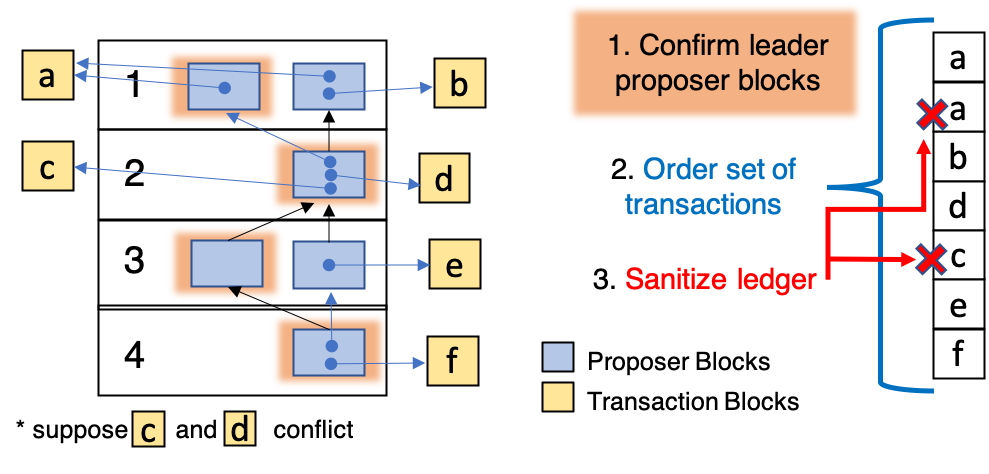
\includegraphics[width=0.75\textwidth]{figures/ledger_generation.png}
    \caption{\small Ledger formation has three parts:  
   (1)  confirming a leader  sequence of proposer blocks;
   (2)  creating a list  of transactions;
   and (3) sanitizing the transaction list for conflicts. 
   In this figure, each transaction  block has only one transaction; suppose transactions  (c) and (d) are inconsistent (e.g., a double spend).
   A proposer block's black reference link denotes a parent link. 
    Blue links denote reference links; a proposer block can include reference links to transaction blocks as well as proposer blocks.}
   %   \gw{A typo: unrefererred $\to$ unreferred? Do we need to use the word unrefererred? Referred blocks are okay in links.}
%   Each shade of grey corresponds to an epoch. In Step 1 (line:\ref{code:txbksOrdering}), all the transaction blocks are incorporated, and in Step 2 (line:\ref{code:sanitizeLedger}), they are combined to build the ledger.
   \label{fig:leader_ledger}

 \end{figure}


\section{Ledger Formation}
\label{sec:confirmation}
% Unlike many blockchain designs, Prism allows transactions to be confirmed before they are ordered. 
% This is possible because confirmation is often an easier task than ordering. 
% For example, consider the following two transactions: a) Alice pays Bob 10\$, and b) Carol pays Drake 10\$. Both these transactions can be individually confirmed without deciding which transaction occurred first.
% The decision to separate transaction confirmation from ordering helps Prism achieve low latency. 
% However, as a result, conflicting or duplicate transactions can become part of the blockchain; these conflicts must be eliminated during transaction ordering (i.e., during ledger formation). 
% % It handles such conflicts by separating the process of confirming blocks and that of generating a ledger from the set of confirmed blocks. 
% % Without it, blockchains must maintain a single, self-consistent sequence of blocks; this causes simultaneously-mined blocks to be wasted, while slowing down the generation of the ledger. 
% % We separately discuss the two procedures of block confirmation and ledger formation. 

% \paragraph{Transaction confirmation}
Prism achieves high throughput in part by mining multiple transaction blocks simultaneously and allowing all of them to contribute to the final ledger. 
A key consequence is that blocks mined concurrently may contain redundant or conflicting transactions.
If Prism were to discard blocks that contain inconsistent transactions, it would needlessly reduce throughput by not confirming the transactions that \emph{are} consistent.
% This would also slow down transaction confirmation, because it means 
To prevent this, Prism separates the process of confirming blocks and forming a ledger. 
This is a key difference between Prism and many other blockchain protocols.
% Since the same transaction can appear in multiple Prism transaction blocks \ma{we need to give more context about why this is a problem. it's all about having a large number of transaction blocks in flight at the same time, so it's fundamentally impossible for a miner to know that a transaction it is mining has not already been included in some other transaction block by another miner}, transaction confirmation is not necessarily the same thing as transaction block confirmation. 
The formation of a ledger in Prism  occurs in three steps, as shown in Figure \ref{fig:leader_ledger}. 

\noindent{\bf (1) Proposer block confirmation.}
First, we must confirm a contiguous sequence of leader proposer blocks at each level.  
    Recall that the proposer block with the most votes on level $\ell$ is defined as the \textit{leader block} at level $\ell$, and the sequence of leader blocks for each level of the proposer tree is defined as the {\em leader sequence}. 
Once we can guarantee that this leader sequence is permanent for all levels up to some level $\ell$ with probability at least $1-\epsilon$, where $\epsilon$ is the target reversal probability, we can confirm a leader block sequence. This process is described in more detail below.

\noindent{\textbf{(2) Transaction  ordering.}}
    Given a proposer block leader sequence, we iterate over the sequence and list the referred transaction blocks in the  order they are referred. 
    We use $L_i$ to denote the leader at level $i$. 
    In Figure \ref{fig:leader_ledger}, we  start  with the leader at level 1 $L_1$, the left proposer block.
    $L_1$ refers to only one transaction  block containing transaction $a$, so our ledger starts with $a$.
    Next, we consider $L_2$. It starts by referring to its parent, the right proposer block at level 1.
    Since that proposer block has not yet been included in the ledger, we include its referred transactions---namely, $a$ and $b$. 
    $L_2$ then adds $L_1$, followed by transaction blocks containing $d$ and $c$, in that order.
    Since $L_1$ was already added to our ledger, we ignore it, but add $d$ and $c$.
    This process continues until we reach the end of our leader sequence.

\noindent{\textbf{(3) Ledger sanitization.}} In the previous step, we may have added redundant or conflicting transactions. 
    Hence, we now execute the transaction list in the previously-specified order. Any duplicate or invalid transactions are discarded. 
    In Figure~\ref{fig:leader_ledger}, we discard the second instance of $a$ (since it's a duplicate), and we discard $c$ (since it conflicts with $d$).

\if 0
\begin{enumerate}
    \item  \textbf{Proposer block confirmation.} First, we must confirm a contiguous sequence of leader proposer blocks at each level.  
    Specifically, the proposer block with the most votes on level $\ell$ is defined as the \textit{leader block} at level $\ell$. 
% This phenomenon is at the core of \schemenosp's security.
The sequence of leader blocks for each level of the proposer blocktree is defined as the {\em leader sequence}. 
Once we can guarantee that this leader sequence is permanent for all levels up to some level $\ell$ with probability at least $1-\epsilon$, we can confirm a leader block sequence. This process is described in more detail below.
    \item \textbf{Transaction  ordering.} 
    Given a proposer block leader sequence, we iterate over the sequence and list the referred transaction blocks in the  order they are referred. 
    We use $L_i$ to denote the leader at level $i$. 
    In Figure \ref{fig:leader_ledger}, we  start  with the leader at level 1 $L_1$, the left proposer block.
    $L_1$ refers to only one transaction  block containing transaction $a$, so our ledger starts with $a$.
    Next, we consider $L_2$. It starts by referring to its parent, the right proposer block at level 1.
    Since that proposer block has not yet been included in the ledger, we include its referred transactions---namely, $a$ and $b$. 
    $L_2$ then adds $L_1$, followed by transaction blocks containing $d$ and $c$, in that order.
    Since $L_1$ was already added to our ledger, we ignore it, but add $d$ and $c$.
    This process continues until we reach the end of our leader sequence.
    \item \textbf{Ledger sanitization.} In the previous step, we may have added redundant or conflicting transactions. 
    Hence, we now execute the transaction list in the previously-specified order. Any duplicate or invalid transactions are discarded. 
    In Figure \ref{fig:leader_ledger}, we discard the second instance of $a$ (since it's a duplicate), and we discard $c$ (since it conflicts with $d$).
\end{enumerate}

\fi
   
%   (3) Iterate over the transactions ledger and \emph{sanitize} it by  removing all  transactions  that conflict with a prior transaction.

% Ultimately, transaction confirmation hinges on confirmation of the proposer blocks that refer to transaction block(s) containing the transaction.
% A transaction block is confirmed once a proposer block pointing to the transaction block is confirmed.
% We thus start by explaining the confirmation of proposer blocks, then explain how this leads to transaction confirmation.


% Specifically, the proposer block with the most votes on level $\ell$ is defined as the \textit{leader block} at level $\ell$. 
% % This phenomenon is at the core of \schemenosp's security.
% The sequence of leader blocks for each level of the proposer blocktree is defined as the {\em leader sequence}. 
% Once we can confirm a contiguous leader sequence, e.g. at levels $1,\ldots, \ell$ with our desired reliability $1-\epsilon$, we can confirm an ordered ledger of transactions. 
% This ledger is formed by iterating over the sequence, and for each leader block, looping over all the transaction blocks referenced within. 
% The list of transactions from each transaction block is added sequentially to the ledger; each transaction's validity is checked for validity (e.g., double spends) and duplicate entries (since the same transaction can be added to multiple transaction blocks). 
% This process is illustrated in Figure \ref{fig:leader_ledger}. \ma{I don't really like Fig. 6. It would be better to create an example which actually shows duplicate transactions and double spends after the ordering step, and than shows the sanitized ledger. BTW, the step of going from ordered transaction blocks to order transactions doesn't seem that important (it's pretty obvious). But the most important point is that you have to do sanitization, and this has to be done after transactions are ordered. }


%\paragraph{Proposer block confirmation.} 
\smallskip
The key to the above confirmation process is leader proposer block confirmation (step 1).
The leader block at a given level $\ell$ can initially fluctuate when the voter trees start voting on level $\ell$. 
However, as the voter trees grow, votes on level $\ell$ are embedded deeper into their respective voter trees, which (probabilistically) prevents the votes from being reverted.
% A leader proposer block at a given level $\ell$ is confirmed based on the votes of the voter trees. 
Hence, we can confirm the leader block when: (1) a plurality of voter trees have voted for it, and (2) that plurality is guaranteed not to change with probability at least $1-\epsilon$, where $\epsilon$ is a user-selected target reversal probability.

%Because there are many voter trees, each individual voter tree needs  only a weak confirmation guarantee to still give a strong confirmation guarantee to the aggregate majority vote. 
% \gw{Do we need to define what is weakly confirm?}

Our confirmation procedure calculates this probability by computing a $(1-\epsilon)$-confidence interval over the number of votes on each leader block, as well as a hypothetical ``private'' block that has not yet been released by a hypothetical adversary that controls a fraction $\beta$ of the hash power. 
Once the leader block's confidence interval is strictly larger than any of the other candidates' confidence intervals, we can be sure (with probability at least $1-\epsilon$) that the current leader will remain the leader for all time, so we confirm that proposer block. 
The details of this confidence interval calculation are included in Appendix~\ref{apx:confirmation}.

\section{Spam Mitigation}
\label{sec:spamming-design}

In Prism, miners do not validate transactions before including them in blocks.
This introduces the possibility of spamming, where an adversary could generate a large number of conflicting transactions and send them to different nodes across the network.  
The nodes would then mine all of these transactions into blocks, causing miners and validators to waste storage  and computational  resources.\footnote{While a discussion of incentives is beyond the scope of this thesis, it is important to note that fees alone cannot prevent such spamming. Assuming nodes only pay for transactions that make it to into the ledger, the adversary would not be charged for conflicting transactions that get removed during sanitization.}
%spam/duplicate transactions
% There are a few practical mechanisms for circumventing this. 
Notice that protocols like the longest chain are not susceptible to this attack because transactions are validated prior to block creation. 
We propose a simple mechanism to mitigate spamming. Miners validate transactions with respect to their latest ledger state and other unconfirmed transactions, giving the adversary only a small window of network delay to spam the system. 
This then allows miners to mitigate spamming attacks by adding a random timing jitter prior to mining transactions, thus increasing the chance that a miner can detect that a conflicting transaction is already present in a transaction block, in  which case it will choose to not include that transaction.
We evaluate the effectiveness of this method in \S\ref{sec:spamming-eval}.

% \smallskip


%We believe such practical countermeasures will be important in  practical settings.
%mitigations:  jitter,  mempool optimization, sortition? 

%\ma{more generally, i think we need to expand this section to explain the important parts of the design in more detail. I don't think the long pseudocode blocks are that helpful. no one will read them, and they don't distinguish the important stuff from the mundane. let's remove the pseudocode to make room to expand on things like: (1) more formal description of block contents (a diagram might help); (2) what exactly is the proof of work puzzle in prism; (3) how does sortition work; (4) how do you get the final block that is sent over the network; (5) how do we get a ledger from all these blocks; (6) how does transaction confirmation work; how and why is it different from bitcoin. there might be other stuff worth mentioning, but we should ideally describe at least each of these points at a decent level of detail} 




% Consider a proposer block sequence from levels $1$ to $\ell$, $\{p_1,\cdots,p_{\ell}\}$, represented by blue blocks in Fig. \ref{fig:leader_ledger}(a).
% Let $L_{p_i}$, represented by green blocks in the grey shaded area in Fig. \ref{fig:leader_ledger}(a), be an ordered list of all the transaction blocks directly or indirectly referred by block $p_i$. 
% Let $\{L_{p_1}, \cdots, L_{p_{\ell}}\}$ be the \textit{transaction block list} of sequence $\{p_1,\cdots,p_{\ell}\}$ as shown in Fig. \ref{fig:leader_ledger}(b). 
% We consider this transaction block list confirmed once each proposer block in the underlying sequence is confirmed. 
% Our proposer block confirmation policy is a simplified version of the policy from \cite{prism}. 
% To confirm a proposer block as leader with reliability parameter $\epsilon$, we consider the votes from all $m$ voter trees. 
% Each voter tree has some maximum probability of ending up with a vote against the block at level $1\leq i \leq \ell$.
% Once we


% While confirming a leader block can take time, 
% we quickly narrow down a set of proposer blocks, defined as the \textit{proposer set}, which is guaranteed probabilistically to contain the eventual leader block for that level. 
% The proposer set is defined as in \todo{XXX--HOW MUCH DETAIL DO WE WANT TO GO INTO? }
% % This procedure first gets all the votes from the voter trees and then gets the proposer set for each 
% % level from the genesis to the last level for which the proposer set can be realized (lines:\ref{code:getvotes_start}-\ref{code:appendPrpList}). 
% Upon  defining a proposer set for each realizable level, Prism takes an outer product of all the proposer sets to  enumerate the set of all possible proposer block leader sequences (line:\ref{code:outerproduct}). 
% Note that by design, one of these sequence will eventually be the leader block sequence.
% It then builds a ledger for each of these proposer block sequences and confirms the given transaction if it is present in \textit{all} of these ledgers (lines:\ref{code:ledgers_for_start}-\ref{code:fastConfirmTx}). 



% \textit{Confirmation and Ordering:} A set of transactions can often be individually confirmed before being ordered among themselves. 
% For this reason, confirming transactions is easier than ordering the transactions.
% For example, consider the following two transactions a) Alice pays Bob 10\$, and b) Carol pays Drake 10\$. Both these transactions can be individually confirmed without deciding which transaction occurred first.
% In Bitcoin, transactions are simultaneously confirmed and ordered; 
% however, in Prism, transactions can be confirmed before being ordered.
% The procedure \textsc{IsTxConfirmed()} in Algorithm \ref{alg:prism_con} defines the transaction confirmation rule $g$ and the procedure \textsc{GetOrderedConfirmedTxs()} defines the rule for ordering the confirmed transactions. Both these procedures use \textsc{BuildLedger()} which is described next.



% \paragraph{Transaction Ordering}
% Once a sequence of leader blocks is confirmed, the ledger is formed by iterating over the sequence, and for each leader block, looping over all the transaction blocks referenced within. 
% The list of transactions from each transaction block is added sequentially to the ledger; each transaction's validity is checked for validity (e.g., double spends) and duplicate entries (since the same transaction can be added to multiple transaction blocks). 
% This process is illustrated in Figure \ref{fig:leader_ledger}(c). 




%\ma{let's move discussion of spamming to the discussion section}
